\documentclass[a4paper,14pt]{article}

\usepackage{comment} % Para comentar várias linhas ao mesmo tempo

%matemática
\usepackage{amsmath}
\usepackage{amssymb}

%diagramação
\usepackage{extsizes}
\everymath{\displaystyle}
\usepackage{geometry}
\usepackage{fancyhdr}
\usepackage{multicol}
\usepackage{graphicx}
\usepackage[brazil]{babel}
\usepackage[shortlabels]{enumitem}
\usepackage{cancel}
\usepackage{textcomp}
\usepackage{tcolorbox}

%tabelas
\usepackage{array} % Para melhor formatação de tabelas
\usepackage{longtable}
\usepackage{booktabs}  % Para linhas horizontais mais bonitas
\usepackage{float}   % Para usar o modificador [H]
\usepackage{caption} % Para usar legendas em tabelas
\usepackage{wrapfig} % Para usar tabelas e figuras flutuantes
\usepackage{xcolor} % Para cores do fundo de tabelas
\usepackage{colortbl} % Para cores do fundo de tabelas

%tikzpicture
\begin{comment}
	\usepackage{tikz}
	\usepackage{scalerel}
	\usepackage{pict2e}
	\usepackage{tkz-euclide}
	\usetikzlibrary{calc}
	\usetikzlibrary{patterns,arrows.meta}
	\usetikzlibrary{shadows}
	\usetikzlibrary{external}
\end{comment}


%pgfplots
\usepackage{pgfplots}
\pgfplotsset{compat=newest}
\usepgfplotslibrary{statistics}
\usepgfplotslibrary{fillbetween}

%colours
\usepackage{xcolor}



\columnsep=2cm
\hoffset=0cm
\textwidth=8cm
\setlength{\columnseprule}{.1pt}
\setlength{\columnsep}{2cm}
\renewcommand{\headrulewidth}{0pt}
\geometry{top=1in, bottom=1in, left=0.7in, right=0.5in}

\pagestyle{fancy}
\fancyhf{}
\fancyfoot[C]{\thepage}

\begin{document}
	
	\noindent\textbf{6FMA107 - Matemática} 
	
	\begin{center}Laboratório de triângulos (Versão estudante)
	\end{center}
	
	\noindent\textbf{Nome:} \underline{\hspace{10cm}}
	\noindent\textbf{Data:} \underline{\hspace{4cm}}
	
	%\section*{Questões de Matemática}
	
	\begin{multicols}{2}
		\noindent Nesta aula, vamos trabalhar com a soma dos ângulos internos de um triângulo. \\
		\noindent\textsubscript{-----------------------------------------------------------------------}
		\begin{enumerate} 
			\item Na ilustração a seguir, complete o que se pede a respeito dos triângulos $ABC$ e $DEF$. Use seu transferidor com bastante cuidado.
			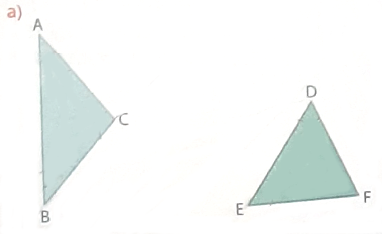
\includegraphics[width=1\linewidth]{6FMA107_imagens/imagem1}
			\begin{itemize}
				\item $m (A\hat{B}C) =$
				\item $m (B\hat{A}C) =$
				\item $m (A\hat{C}B) =$
				\item $m (D\hat{E}F) =$
				\item $m (E\hat{D}F) =$
				\item $m (D\hat{F}E) =$
			\end{itemize}
			Calcule a soma dos três ângulos em cada triângulo. A que conclusão você chegou?
			\begin{enumerate}[b)]
				\item Verifique mais uma vez esse resultado para o triângulo a seguir: \\
				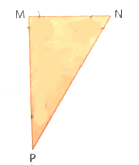
\includegraphics[width=1\linewidth]{6FMA107_imagens/imagem2}
				\begin{itemize}
					\item $m (M\hat{N}P) =$
					\item $m (N\hat{M}P) =$
					\item $m (N\hat{P}M) =$
				\end{itemize}
			\end{enumerate}
			\item Em uma folha de papel, desenhe um triângulo qualquer e pinte os seus três ângulos com cores diferentes. Em seguida, recorte o triângulo em três regiões, de forma que cada ângulo fique em um pedaço. \\
			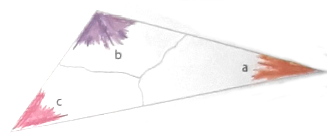
\includegraphics[width=1\linewidth]{6FMA107_imagens/imagem3}
			Una os três ângulos em um mesmo vértice, da seguinte forma: \\
			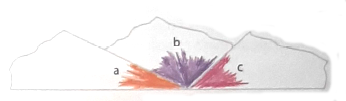
\includegraphics[width=1\linewidth]{6FMA107_imagens/imagem4}
			Descreva com suas palavras o que aconteceu.
			Podemos então concluir que $a + b + c = \underline{~~~~~~~~}°$.
			\item Calcule $x$ em cada uma das figuras a seguir. \\
			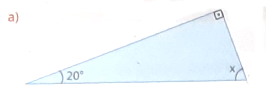
\includegraphics[width=1\linewidth]{6FMA107_imagens/imagem5}
			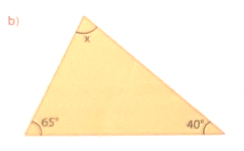
\includegraphics[width=1\linewidth]{6FMA107_imagens/imagem6}
			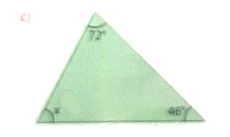
\includegraphics[width=1\linewidth]{6FMA107_imagens/imagem7}
			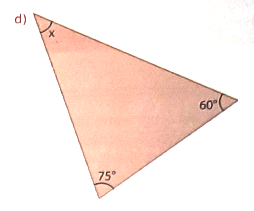
\includegraphics[width=1\linewidth]{6FMA107_imagens/imagem8}
			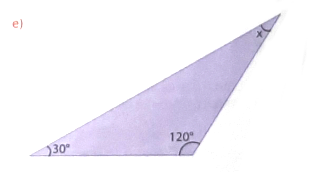
\includegraphics[width=1\linewidth]{6FMA107_imagens/imagem9}
			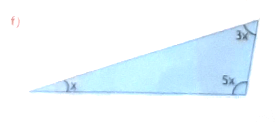
\includegraphics[width=1\linewidth]{6FMA107_imagens/imagem10}
			%75 a 76
			\item Calcule a medida do ângulo $A\hat{B}C$ nos triângulos a seguir. \\
			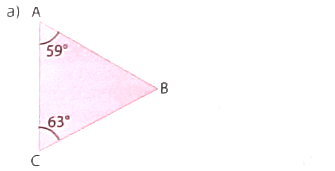
\includegraphics[width=1\linewidth]{6FMA107_imagens/imagem11}
			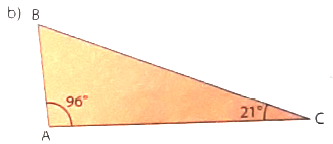
\includegraphics[width=1\linewidth]{6FMA107_imagens/imagem12}
			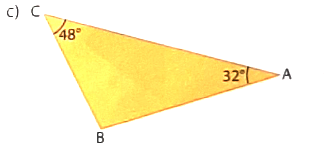
\includegraphics[width=1\linewidth]{6FMA107_imagens/imagem13}
			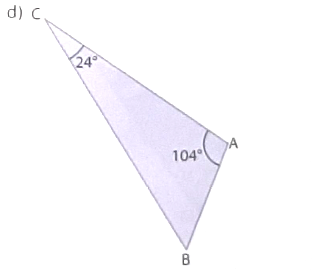
\includegraphics[width=1\linewidth]{6FMA107_imagens/imagem14}
			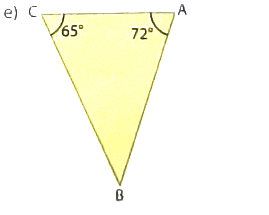
\includegraphics[width=1\linewidth]{6FMA107_imagens/imagem15}
			\item Dados dois ângulos de um triângulo, determine o terceiro em cada caso.
			\begin{enumerate}[a)]
				\item 34° e 62°.
				\item 27° e 73°.
				\item 105° e 18°.
				\item 93° e 36°.
				\item 121° e 47°.
				\item 81° e 26°.
			\end{enumerate}
		\end{enumerate}
		$~$ \\ 	$~$ \\ 	$~$ \\ 	$~$ \\ 	$~$ \\ 	$~$ \\ 	$~$ \\ 	$~$ \\ 	$~$ \\ 	$~$ \\ 	$~$ \\ 	$~$ \\ 	$~$ \\ 	$~$ \\ 	$~$ \\ 	$~$ \\ 	$~$ \\ 	$~$ \\ 	$~$ \\ 	$~$ \\ 	$~$ \\ 	$~$ \\ 	$~$ \\ 	$~$ \\ 	$~$ \\ 	$~$ \\ 	$~$ \\ 	$~$ \\ 	$~$ \\ 	$~$ \\ 	$~$ \\ 	$~$ \\ 	$~$ \\ 	$~$ \\ 	$~$ \\ 	$~$ \\ 	$~$ \\ 	$~$ \\ 	$~$ \\ 	$~$ \\ 	$~$ \\ 	$~$ \\ 	$~$ \\ 	$~$ \\ 	$~$ \\ 	$~$ \\ 	$~$ \\ 	$~$ \\ 	$~$ \\ 	$~$ \\ 	$~$ \\ 	$~$ \\ 	$~$ \\ 	$~$ \\	$~$ \\ 	$~$ \\ 	$~$ \\ 	$~$ \\ 	$~$ \\ 	$~$ \\ 
	\end{multicols}
\end{document}